\documentclass[
	a4paper,
	twoside,
	11pt,
	numbers=noenddot, 				% No dot after numbers for chapters, sections, etc.
	cleardoublepage=empty, 			% Left plain page before chapters
	%DIV=15,            			% Adjust this value for more/less text on pages
	BCOR=5mm 						% Binding correction
]{scrbook}

%%%%%%%%%%%%%%%%%%%%%%%%%%%%%%
%%%%%%%%%% Preamble %%%%%%%%%%
%%%%%%%%%%%%%%%%%%%%%%%%%%%%%%

% Kopf- und Fusszeile
\usepackage[manualmark]{scrpage2} 	% Package scrpage2 erlaubt es die Kopf- und Fußzeile zu gestalten. Optionen sind automark oder manualmark
\pagestyle{scrplain}				% Nur Seitenzahl in Fußzeile. Sonst bleibt Kopf- und Fußzeile leer. Mit "headings" wird Kopf- und Fußzeile eingebunden
\ofoot[]{} 							% Seitenzahl am Rand wird nur gesetzt wenn \pagemark eingefügt wird. Wenn es leer bleibt wird nichts geschrieben
\cfoot[\pagemark]{\pagemark} 		% Seitenzahlen in der Seitenmitte, wenn \pagemark eingefügt. Ansonsten keine Seite

\setlength{\parindent}{0pt} 		% Indent ist set to the given value

% Sprache
\usepackage[english, german]{babel}
\usepackage{verbatim} 				% Text in the env "comment" is interpreted as a comment

% mathematical packages
\usepackage{amsmath}
\usepackage{mathtools}
\usepackage{amssymb}
\usepackage{physics} 				% Usefull package for physical and mathematical formulas. Package-documentation: http://ftp.fau.de/ctan/macros/latex/contrib/physics/physics.pdf

% package for including graphics
\usepackage{graphicx}
\usepackage{subfigure} 				% Package for setting two graphics side by side
\usepackage{epstopdf} 				% Convert eps-files to pdf-files
\graphicspath{{figures/}} 			% Path to all figures used in this document

\usepackage{bm}						% Make the argument bold
\usepackage{xcolor}					% Package for changing he color of letters, numbers and other things 
\usepackage{float}					% Improve interface of floating objects

\usepackage{enumitem} 				% change the level in enumerate-envirement

\usepackage[draft]{todonotes}   	% draft: notes showed, disable: not showed

% bibiography package and stylesetting
\usepackage[
	backend = biber, 
	bibencoding = utf8,
	style = alphabetic, 
	sorting = none, 
	autocite = plain, 
	language = autobib,
]{biblatex} 
\addbibresource{bibliography/masterthesis.bib}
\usepackage{csquotes}
%\usepackage{hyperef}
%\hypersetuo{
	%draft,							% De-activate all hyperref settings
	%linkcolor=red,					% Internal links are red
	%citecolor=green,				% Citations are green
	%urlcolor=cyan					% url-links are cyan
	%colorlinks=true					% Links are colorfull
%}
%

%%%%%%%%%%%%%%%%%%%%%%%%%%%%%%%%%%%%%%%%%
%%%%%%%%%% self-defined macros %%%%%%%%%%
%%%%%%%%%%%%%%%%%%%%%%%%%%%%%%%%%%%%%%%%%

\newcommand{\mt}[1]{\mathrm{#1}} %%% text in math-mode get normal like you aren't in math-mode

%%% braket notation in the hilbertspace of operators (Liouville space) %%%

\newcommand{\oket}[1]{\big|{#1}\big)} % ket in operator space with automatic sizing
\newcommand{\toket}[1]{|\mt{#1})} % ket in operator space for writing inside normal text

\newcommand{\obra}[1]{\big({#1}\big|} % bra in operator space with automatic sizing
\newcommand{\tobra}[1]{(\mt{#1}|} % bra in operator space for writing inside normal text

\newcommand{\obraket}[2]{\big({#1}\big|{#2}\big)} % braket in operator space with automatic sizing
\newcommand{\tobraket}[2]{({#1}|{#2})} % braket in operator space for writing inside normal text

\newcommand{\odyad}[2]{\oket{#1}\obra{#2}} % dyad in operator space with autometic sizing
\newcommand{\tdyad}[2]{\toket{#1}\tobra{#2}} % dyad in operator space for writing inside normal text

%\newcommand{\ev}[1]{\left\langle{#1}\right\rangle} 											% expactation value
%\newcommand{\erwartungswert}[3]{\left\langle {#1}\right|{#2}\left|{#3}\right\rangle} 		% ausführlicher erwartungswert mit zuständen
%\newcommand{\kom}[2]{\Big[{#1},{#2}\Big]} 													% commutator
%\newcommand{\antikom}[2]{\Big\{{#1},{#2}\Big\}} 											% anticommutator
%\newcommand{\integral}[4]{\int\limits_{{#1}}^{{#2}}{#3}\ {#4}} 								% integral: #1->lower limit; #2->upper limit; #3->differential operator; #4->integrand
%\newcommand{\scalarproduct}[2]{\left({#1}|{#2}\right)} 										% scalar product super operator
%\newcommand{\opnorm}[1]{\left({#1}|{#1}\right)} 											% norm super operator
%\newcommand{\evso}[3]{\left({#1}\right|{#2}\left|{#3}\right)} 								% expactation value super operator
%\newcommand{\projectionoperator}[2]{\frac{\left|{#1}\right)\left({#2}\right|}{\opnorm{#2}}} % projectionoperator super operator
%\newcommand{\opket}[1]{\left|{#1}\right)} 													% operator ket
%\newcommand{\opbra}[1]{\left({#1}\right|} 													% operator bra
%\newcommand{\trace}[1]{\mathrm{Tr}\left\{{#1}\right\}} 										% trace
%\newcommand{\green}[2]{\big\langle\big\langle{#1};{#2}\big\rangle\big\rangle} 				% Definition of Green-function with angle brackets
%\newcommand{\totalDif}[1]{\frac{\mathrm{d}}{\mathrm{d}{#1}}} 								% totale differentiation
%\newcommand{\partialDif}[1]{\frac{\partial}{\partial{#1}}} 									% partielle differentiation
%\newcommand{\longkom}[2]{\Big[{#1},\vphantom{\Big]}\notag\\\vphantom{\Big[}&{#2}\Big]} 		% commutator with linebreak between #1 und #2
%\newcommand{\longev}[2]{\Big\langle{#1}\\ &{#2}\Big\rangle}									% expectation value with linebreak between #1 and #2

% Vectors and matricies
%\newcommand{\bvec}[1]{\textbf{#1}} 															% vector bold letter
%\newcommand{\oneTwoVec}[2]{\begin{pmatrix}#1 & #2\end{pmatrix}} 							% two componand row vector
%\newcommand{\twoOneVec}[2]{\begin{pmatrix}#1\\#2\end{pmatrix}} 								% two componand column vector
%\newcommand{\twoTwoMatrix}[4]{\begin{pmatrix}#1 & #2\\#3 & #4\end{pmatrix}} 				% 2x2 matrix

% Fourier transformation
%\newcommand{\fouriertrafo}[4]{\int \frac{\mathrm{d}^{#4}{#3}}{(2\pi)^{#4}}\, {#1}({#3},\tau) e^{#2}} % Fouriertrafo into momentum space (#1: function; #2: argument of e; #3: momentum letter; #4: dimension)

% definition of mathematical functions
\DeclareMathOperator{\sign}{sign}
%\DeclareMathOperator{\Real}{Re}
%\DeclareMathOperator{\Imag}{Im}

%%%%%%%%%%%%%%%%%%%%%%%%%%%%
%%%%%%%%%% Layout %%%%%%%%%%
%%%%%%%%%%%%%%%%%%%%%%%%%%%%








%%%%%%%%%%%%%%%%%%%%%%%%%%%%%%%%%%%%%%%%%%%%%%%
%%%%%%%%%% Beginning of the document %%%%%%%%%%
%%%%%%%%%%%%%%%%%%%%%%%%%%%%%%%%%%%%%%%%%%%%%%%

\begin{document}

\pagestyle{empty}					% no pagestyle -> no heading, no numbering
\selectlanguage{german}				% document language set to german

%%% Your personal titlepage in german
%%% Can be used for diplomathesises
%%%
%%% adjust all the red colored text and remove the color tags

\begin{titlepage}
  \rmfamily
  \begin{center}
    { \Large
      \hrule
      \vspace{1em}
      \begin{center}

        \begin{minipage}[hbt]{4cm}
          \centering
          
\includegraphics[draft=false, width=3cm]{logos/KITlogo_transparent.eps}
        \end{minipage}
        \begin{minipage}[hbt]{11cm}
          Fakult"at f"ur Physik

          Institut f"ur Theorie der Kondensierten Materie
        \end{minipage}
      \end{center}
      \vspace{1em}
      \hrule 
    } 
    \vspace*{\stretch{11}}
    { 
      \LARGE\bfseries
      Quantentransport in Spindichtesystemen mit dem Memory-Matrix-Formalismus\\       
    }
    \vspace*{\stretch{14}}
    {
      %\includegraphics[width=10cm]{Titlepage/cover}\\
    }
    \vspace*{\stretch{8}}
    { \Large
      Masterthesis \\
      \vspace*{\stretch{0.5}}
      von \\
      \vspace*{\stretch{0.5}}
      Martin Lietz\\
    }
    \vspace*{\stretch{2}}
    { \large 
      27.\,Mai\,2017 bis 27.\,Mai\,2018\\
    }
    \vspace*{\stretch{5}}
    { \large
      \begin{tabular}{r@{\hspace{2em}}l}
        Referent:     & Prof.\,Dr.\,J"org Schmalian\\
        Korreferent:  & Prof.\,Dr.\,Alexander Shnirman
      \end{tabular}
    }
  \end{center}
  \vspace*{\stretch{1}}
\end{titlepage}
\cleardoublepage
		% titlepage in german
%%%% Your personal titlepage in german
%%% Can be used for diplomathesises
%%%
%%% adjust all the red colored text and remove the color tags

\begin{titlepage}
  \rmfamily
  \begin{center}
    { \Large
      \hrule
      \vspace{1em}
      \begin{center}

        \begin{minipage}[hbt]{4cm}
          \centering
          
\includegraphics[draft=false, width=3cm]{logos/KITlogo_transparent.eps}
        \end{minipage}
        \begin{minipage}[hbt]{11cm}
          Fakult"at f"ur Physik

           Institut f"ur Theorie der Kondensierten Materie
        \end{minipage}
      \end{center}
      \vspace{1em}
      \hrule 
    } 
    \vspace*{\stretch{11}}
    { 
      \LARGE\bfseries
      Vector $\phi^4$-model in hyperbolic space\\       
    }
    \vspace*{\stretch{14}}
    {
      %\includegraphics[width=10cm]{Titlepage/cover}\\
    }
    \vspace*{\stretch{8}}
    { \Large
      Master's Thesis \\
      \vspace*{\stretch{0.5}}
      by \\
      \vspace*{\stretch{0.5}}
      Alexander Gawrilow\\
    }
    \vspace*{\stretch{2}}
    { \large 
      January 24, 2017 - January 24, 2018\\
    }
    \vspace*{\stretch{5}}
    { \large
      \begin{tabular}{r@{\hspace{2em}}l}
        Advisor:     & Prof.~Dr.~J"org Schmalian\\
        Co-Advisor:  & Prof.~Dr.~Alexander~Shnirman
      \end{tabular}
    }
  \end{center}
  \vspace*{\stretch{1}}
\end{titlepage}
\cleardoublepage
		% titlepage in english

\frontmatter						% activate roman numbering
\pagestyle{plain}

\cleardoublepage
\vspace*{30\baselineskip}
%\hbox to \textwidth{\hrulefill}
\par
\noindent {Ich erkl"are hiermit, dass die Arbeit selbstst\"andig angefertigt, alle benutzten Quellen und Hilfsmittel vollst\"andig und genau angegeben und alles kenntlich gemacht wurde, das aus Arbeiten anderer unver\"andert oder mit Ab\"anderungen entnommen ist.
}
\vspace{1cm}

\noindent
Karlsruhe, den \today{}

\vspace{1cm}

\noindent\dotfill\hspace*{10.0cm}\\
(\textbf{Martin Lietz}) %center name with hspace
		% assertion in german

\selectlanguage{english}			% document language set to english
\cleardoublepage
%
%
\chapter*{Acknowledgment}
%
%
%I would like to express my thanks to my advisor J\"org Schmalian who encouraged and supported me and gave the right hints at the right time during the last year. 
%His essential input lead to the results presented in this work. 

%Furthermore, I would like to thank Una Karahasanovic for all the discussions and information which became decisive for one topic of this work. 

%Then, I have to thank especially Jian Kang who crucially contributed to the discussion of bond currents and Rafael Fernandes for the fruitful discussions on the general topic. 

%Special thanks to all the colleagues of the condensed matter group at the KIT. Especially to Bhilahari Jeevanesan for all the discussions and help with several problems and to Pablo Schad for finalizing this work. 

%Last but not least, I have to thank my family, my mother and sister and especially Anja for all the support and encouraging words. 
 
		% help from colleagues and friends

\cleardoublepage
\tableofcontents					% table of contents

\pagestyle{scrheadings}				% activate heading and numbering
\mainmatter							% activate	arabic numbering

% includeing chapters
\cleardoublepage
\chapter{Motivation}

%
\cleardoublepage
%
%
%
\chapter{Spin-Fermion-Model}
\label{ch: spin fermion model}
%
%
%
In the following chapter the spin-fermion-model for a metal exhibiting a antiferromagnetic quantum phase transition is introduced as presented in \cite{Abanov&Chubukov&Schmalian}.
Beside fermionic particle-hole-exitetaions in the vicinity of the quantum critical point bosonic spin fluctuations arise in this low energy theory, which enable a attractive interaction between electrons.
This chapter isn't displayed a detailed mathematical or microscopic derivation of the spin-fermion-model, but rather it is based on a qualitative description to justified its form.
For that a shortly overview over quantum phase transitions are established as suggested in \cite{SachdevQCP}.
In particular, we focus one's attention on the arising spin fluctuations, agrue them carry large momenta and introduced the damped spin density propagator and their perodicity.
Further we present the basic concepts of hot-spot theory, which are points on the Fermi surface in 2D emerged since the magnetic Brillouin zone cutting the Fermi surface.
Besides we review explicitly the conservation of momentum and non-conservation of current for the observing Hamiltonian.
For breaking translation symmetry umklapp scattering is introduced and we prove that this is unconserving momentum.
%
%
\section{Spin-Fermion-Model}
\label{sec:spin-fermion-model}
%
%
Many metals exhibit an antiferromagnetic phase transition at a characteristic temperature $\mt{T}_{\mt{N}}$, called N\'eel-temperature.
The random ordered spins of lattice atoms ordering in consequence of thermal fluctuations along one axis, where the nearest neighbors are always aligned in opposite direction.
This temperature can be changed by tuning a certain parameter like pressure or doping, for example.
A schematic and simplified phase diagram is depicted in figure \ref{fig:phase diagram}.
%
\begin{figure}[t]
	\centering
	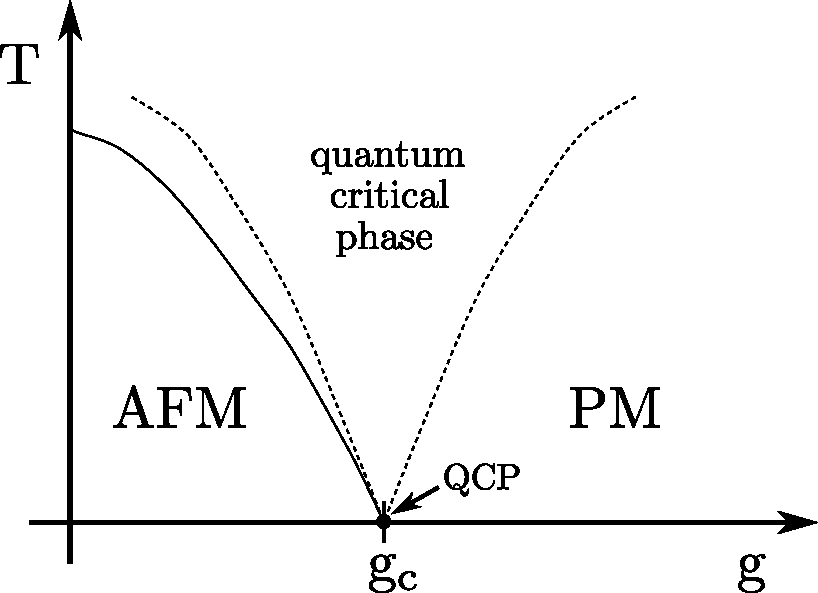
\includegraphics[width=0.7\textwidth]{phase_diagram.pdf}
	\caption{
This figure shows a schematic and simplified phase diagram for metals transition from a paramagnetic (PM) into an antiferrmagnetic (AFM) phase depending on a tunung parameter g.
The phase line of the AFM phase ends decreasing temperature down to $T = 0$ in a quantum critical point (QCP) at $\mt{g} = \mt{g}_{\mt{c}}$.
At this point the phase transition is only caused by quantum fluctuations.
At $T > 0$ thermal fluctuactions more and more dominates the phase transition.
Nevertheless quantum fluctuations influences the physical behaviour in a lagre regime, labeled as quantum critical phase.
	}
	\label{fig:phase diagram}
\end{figure}
%
Decreasing tempearutre the phase line between both magnetic phases reach a certain value for the tuning parameter g at $T = 0$, labeled with $\mt{g}_{\mt{c}}$.
This point is called quantum critical point and in comparsion with the phase transition at finite temperature quantum fluctuations are the origin of this phase transition.

Before starting with a qualitative derivation of the spin-fermion-model a short and rudimentary describtion of quantum phase transition is given.
This overview is required for the analytical discussion of our computation later.
However, the reason for phase transitions is always level crossing between the ground and an excited state.
Due to the fact that level crossing is forbidden a band gap $\Delta$ arises.
This band gap is therefore a characteristic energy scale of the quantum phase transition.
Considering only phase transitions of second order the characteristic energy scale $\Delta$ is proportional to the tuning parameter as
%
\begin{align}
	\Delta \sim \mt{J} |\mt{g} - \mt{g}_{\mt{c}}|^{z \nu},
	\label{eq:energy scale Delta}
\end{align}
%
where $z\nu$ is a critical exponent and J a energy scale of a microscopic coupling \cite{SachdevQCP}.
Beside a characteristic energy scale quantum phase transitions also possesses a characteristic length scale $\xi$, called correlation length, which diverges right at the quantum critical point.
%
\begin{align}
	\xi^{-1} \sim \Lambda |\mt{g} - \mt{g}_{\mt{c}}|^{\nu},
	\label{eq:correlation length xi}
\end{align}
%
where $\nu$ is again a critical exponent and $\Lambda$ an arbitrary inverse length scale like a momentum cut-off, for example.
Inserting \eqref{eq:correlation length xi} in \eqref{eq:energy scale Delta} yields a directly relation between both characteristic quantities.
For finite temperatures, $T > 0$, a second energy scale is given by $k_{\mt{B}} T$, where $k_{\mt{B}}$ is the Botzmann constant.
Comparing both energy scales yields a proportionality between temperatur and correlation length as
%
\begin{align}
	T \sim \xi^{-z}.
	\label{relation temperature and correlation length}
\end{align}
%
Further this explaines the curved conical boundary phase lines of the quantum critical phase in figure \ref{fig:phase diagram}.
In the case of small temperatures the critical exponent $z$ attains the value $z = 2$, so that the phase lines are shaped like a square root.
Increasing temperature the phase boundary lines are linear, since the critical exponent changing to $z = 1$ \cite{Patel&Sachdev}.
Inside this regime the physical behaviour of the metals is determined by quantum fluctions.

Knowing the physical origin of quantum phase transitions the spin-fermion-model can be introduced.
Instead of an microscopic and detailed mathematical describtion we want focus our introduction on qualitative arguments motivating the model.
The spin-fermion-model describes metals in the vicinity of a magnetic quantum critical point considering fermionic quasiparticles and bosonic spin density waves.
Thereby, the propagator is determined by the usual free fermionic Green function.
Spin fluctuations are constituted as collective modes and their propagator is characterized by the dynamical magnetic susceptibility.
%
\begin{align}
	\mathcal{D}_{\mu}(\vb{q}, \omega) = \sum\limits_{\vb{Q}} \frac{1}{(\vb{q}+\vb{Q})^{2} + \xi^{-2} - (\flatfrac{\omega}{v_{\mt{S}}})^{2}},
	\label{eq:undamped spin propagator}
\end{align}
%
where $\mu$ is the spatial direction of the spin density wave, $\xi$ the magnetic correlation length and $v_{\mt{S}}$ the spin wave velocity.
The spin wave velocity is of the same order as the Fermi velocity since spin fluctuations originate due to fermions in the vicinity of the Fermi surface.
Furthermore, the magnetic susceptibility possesses a peak at the momentum vector $\vb{Q} = (\pi, \pi)$.
This implicates a strong coupling interaction between momentum vectors $\vb{k}$ and $\vb{k} + \vb{Q}$.

Phase transitions are always associated by an order parameter equally the investigated antiferromagnetic phase transition, where the local magnetization measured by the spin expectation value $\expval{\mt{S}_{\mu}}$ is the corresponded one.
Similar to the propagator the index $\mu$ indicated the spatial direction.
The order parameter is finite in the antiferromagnetic ordered phase and reaches zero in the paramagnetic disordered phase.
Further, the expectation value of the spin operator is spatially modulated according to $\expval{\mt{S}_{\mu}} \sim e^{i\vb{Q}\vb{R}}$, where $\vb{R}$ is some lattice vector \cite{Weiss}, and therefore the order parameter and equally the propagator are periodical quantities.
In reciprocal space this is reflected in the periodicity  of the magnetic Brillouin zone spanned by the vector $\vb{Q}$.

Our describtion of the antiferromagnetic quantum phase transition in the spin-fermion-model is based on a few fundamental assumptions, comparatively to \cite{Abanov&Chubukov&Schmalian}.
We assume spin fluctuations arise over a large range of the tuning parameter and other low-energy collective degrees of freedom, independent on spin excitations, are neglectable.
Starting by large values of the tuning parameter g, where the metal is in the paramagnetic phase, the physical behaviour is described by Landau's Fermi liquid theory.
Decreasing the tuning parameter and getting closer to the quantum critical point changes the behaviour of the Fermi liquid.
Assuming only one type of fermions the arising collective modes are originated due to permanent interaction between particles and holes.
These bosonic spin excitations determine the physics in the vicinity of the quantum critical point and turning into smooth modes.
Therefore, we assume that only one dominant channel exist for fermion-fermion interaction with energies smaller than an energy cut-off $\Lambda$.
Further we introduce on collective spin mode which containts this interaction.
\todo{Diesen Abschnitt nochmal \"uberarbeiten}
The obtained effective Hamiltonian for the spin fluctuations in the low-energy theory is given by
%
\begin{align}
	\mt{H}_{\Phi} &= 
	 	\int_{\vb{k}}\, \Big[-\frac{\vb{k}^{2}}{2} - \frac{r}{2}\Big] \Phi_{\mu}(\vb{k},\tau) \Phi_{\mu}(-\vb{k},\tau)
		+
		\frac{v_{\mt{S}}^{2}}{2} \pi_{\mu}(\vb{k},\tau) \pi_{\mu}(-\vb{k},\tau)
	\label{eq:Hamiltonian spin fluctuation}
\end{align}
%

In two dimensions the dimensionless coupling constant $\lambda$ is proportional to the inverse magnetic correlation length $\xi$ and diverges at the quantum critical point.



















%
\cleardoublepage
%
%
\chapter{Memory-Matrix-Formalsim}
\label{ch: memory-matrix-formalism}
%
%
\section{Motivation}
\label{sec: motivation}
%
%
A physicist is always interested in the beaviour and time evolution of the observables of the investigates system.
In the middle of the last century many physicists worked on the understanding and mathematical description of one physical process, the Brownian motion.
On stochasical theory of these certain physical process is based on the Langevin equation
%
\begin{align}
	\pdv{t} \mt{A}(t) -\mt{F}_{\mt{ex}}(x,t) + \gamma \cdot \mt{A}(t) = f(t),
	\label{eq: Langevin equation}
\end{align}
%
where $\mt{A}(t)$ is some dynamical observable and $f(t)$ is a random force like white noise for example.
The origin of the second term on the left hand side is some external force result from a coupling between $\mt{A}(t)$ and some external potential.
The third term on the left hand side is a damping or friction term.
Now let us assume it's possible to seperate equation \eqref{eq: Langevin equation} into two parts.
The first part, called $f_{1}$, is a functional of the dynamical observable $\mt{A}(t')$, where $t_{0} \leq t' \leq t$, so that this part is depending on the history of A.
The second part $f_{2}$ should be depending on all other degrees of freedom.
Now $f_{1}$ is expanded up to the linear order and all terms of higher order and the part $f_{2}$ are summerized to the quantity $F(t)$.
The result is a linearized form of the Langevin equation
%
\begin{align}
	\pdv{t} \mt{A}(t) = \int\limits_{t_{0}}^{t} \dd{t'} \mathcal{C}(t-t') \mt{A}(t') + F(t),
	\label{eq: linearized Langevin equation}
\end{align}
%
where $\mathcal{C}$ is a correlation function and $\mt{A}(t')$ is the deviation of the invariant part of the Hamiltonian.
For large time scales the deviation should be vanish, so the time-integral over $\mt{A}(t')$ should be become zero.
For simplification the origin of the time axis is moved to $t_{0}$.
In general the Laplace transformation of a function is given by
%
\begin{align}
	\mathcal{L}\big\{\mt{A}(t)\big\} = \mt{A}(s) = \int\limits_{0}^{\infty} \dd{t} \mt{A}(t) e^{-st}.
	\label{eq: Laplace transformation real axis}
\end{align}
%
Using the Laplace transformation equation \eqref{eq: linearized Langevin equation} becomes a algebratic equation of motion.
The solution of this equation is 
%
\begin{align}
	\mt{A}(t) = \Xi(t) \cdot \mt{A}(0) + \mt{A}'(t) \hspace{1cm} \mt{with} \hspace{1cm} \mt{A}'(t) = \int\limits_{0}^{t} \dd{t'} \Xi(t-t') F(t'),
	\label{eq: splitted observable}
\end{align}
%
where the function $\Xi(t)$ is defined by the Laplace transformation of $\Xi(s) = [s-\mathcal{C}(s)]^{-1}$ and $\mathcal{C}(s)$ is the Laplace transformtion of the correlation function $\mathcal{C}(t)$.
The main result of equation \eqref{eq: splitted observable} and the motivation for the following introduced memory-matrix-formalism is the splitting of the dynamical observable $\mt{A}(t)$ into two parts.

For the first term on the right hand side the only time-dependence is adverted through the correlation function $\mathcal{C}$, which is clear regarding the definition of $\Xi$.
This term included the linear contributions of $\mt{A}(t)$ by construction.
These ones are the mostly important contributions to the time evolutaion of an observable, because they are secular.
In contrast the second term on the right hand side is the convolution between the function $\Xi(t-t')$ and the function $\mt{F}(t')$.
The latter summerize all the non-linear effects, fluctuations and intital transient processes, which are all effects with a small lifetimes in contrast with the secular effects.
Therefore these effects shouldn't have large influences on the time evolution of an observable, always large time scales in mind.

Beside the physical interpretation a simple geometrical and mathematical one is very usefull.
Let us assume a vector space ana the observable should be a vector in this vector space.
Then the secular term is a projection on the A-axis and the non-secular term is aquivalent to a vector perpendicular to the A-axis.
The memory-matrix-formalism take up this simple interpretation of equation \eqref{eq: splitted observable} and put it in a general and exact form, so that it can be used classicaly and quantum mechanicaly.
%
%
\section{Linear Response Theory}
\label{sec: linear response theory}
%
%
Before the derivation of the memory-matrix-formalism can be started some ground work is to do.
This section begins with a short reminder of the kubo formula. %also known as linear response theory.
After that the Kubo relaxation function are introduced and some important relations between there and the retarded susceptibility $\chi$ are derivated.
In the last section finally the splitting of $\chi$ in a real and an imaginary part are dicussed.
%
%
\subsection{Kubo formula}
\label{subsec: kubo formula}
%
%
Consider a system in equilibrium represented by the Hamiltonian $H_{0}$.
At an arbitrary time $t'$ a pertubation is switched on, where the pertubation is given by the Hamiltonian $H_{1} = - B \cdot F(t)$, so that $H(t) = H_{0} + H_{1}$ is the full Hamiltonian.
Thereby $B$ is an operator by which the pertubation is coupled on the system and $F(t)$ is a function determining the time evolution of the pertubation.
It is assumed that $F(t) = 0$ for $t<t'$ so that the system is in thermal equilibrium for all these times.

The physical interest is existed in the question how does an observable $\mt{A}$ react on the pertubation switched on at $t'$.
The answer is given by the thermodynamical expectation value of the operator corresponding to the observable $\mt{A}$
%
\begin{align}
	\expval{\mt{A}}(t) := \Tr{\rho_{\mt{S}}(t) \mt{A}_{\mt{S}}} = \Tr{\rho_{\mt{I}}(t) \mt{A}_{\mt{I}}},
	\label{eq: thermodynamical expectation value}
\end{align}
%
where the label S and I stand for the Schrödinger and Interaction picture, respectivily.
The equality of the expectation value in the different regarded pictures is shown by the invariance of the trace under cycle permutation.
The transformation into the interaction picture is very usefull what we will see after the next step below.
In quantum mechnics the time evolution of the density operator is determined by the von Neumann-equation.
%
\begin{align}
	\dv{t} \rho_{\mt{S}}(t) = -\frac{i}{\hbar} \comm{H(t)}{\rho_{\mt{S}}(t)} \hspace{0.5cm}\Leftrightarrow\hspace{0.5cm} \dv{t} \rho_{\mt{I}}(t) = -\frac{i}{\hbar} \comm{H_{1}}{\rho_{\mt{I}}(t)}
	\label{eq: von Neumann-equation}
\end{align}
%
The equation is also transformed into the interaction picture, which doesn't change the structure itself but the density operator deponds only on the Hamiltonian $H_{1}$ now.
Integrating and using the boundary condition that the system is in thermal equilibrium at $t \to -\infty$ equation \eqref{eq: von Neumann-equation} is resulted in a integrable equation for the density operator.
%
\begin{align}
	\rho_{\mt{I}}(t) = \rho_{0} + \frac{i}{\hbar} \int\limits_{-\infty}^{t} \dd{t'} \comm{B_{\mt{I}}(t')}{\rho_{\mt{I}}(t')}F(t')
	\label{eq: integrable form of von Neumann-equation}
\end{align}
%
Jet it is clear why the interection picture is used.
The integrand depends on the Hamiltonian of the pertubation only in linear order which is a perfect starting point for a iterativ solution procedure.
Starting with the zeroth order the density operator is trivially the density operator at thermical equilibrium.
Inserting the zeroth order on the right hand side of equation \eqref{eq: integrable form of von Neumann-equation} yield the first order of the density operator, a.\,s.\o.
In linear response theory the iteration is cutted off after the first order.
Inserting this in equation \eqref{eq: thermodynamical expectation value} and defining the dynamical susceptibility 
%
\begin{align}
	\chi_{\mt{AB}}(t-t') = \frac{i}{\hbar} \Theta(t-t') \expval{\comm{A_{\mt{I}}(t-t')}{B_{\mt{I}}(0)}}_{H_{0}}
	\label{eq: dynamical susceptibilty}
\end{align}
%
yield the Kubo formula
%
\begin{align}
	\delta\expval{\mt{A}(t)} := \expval{\mt{A}}(t) - \expval{\mt{A}(t)}_{H_{0}} \approx \int\limits_{-\infty}^{\infty} \dd{t'} \chi_{\mt{AB}}(t-t') F(t'),
	\label{eq: Kubo formula}
\end{align}
%
where the label $H_{0}$ means that the expactation value is taken with respect to the unpertubated Hamiltonian.
We see that the deviation of the observable A caused by the pertubation is given by the convolution of the dynamical suszeptibilty $\chi_{\mt{AB}}(t-t')$ and the time evolution function $F(t)$.\todo{noch sch\"oner schreiben}
%
%
\subsection{Kubo relaxation function}
\label{subsec: Kubo relaxation function}
%
%
After a general equation for the deviation of an observable A from the equilibrium value was established, we want to investigate a certain kind of pertubation.
Let us assume $F(t) = \Theta(-t) \cdot F \cdot e^{-s\tau}$ the time evolution function of a pertubation, which is switched on adiabatically at $t=-\infty$ and switched off at $t=0$.
Inserting this in equation \eqref{eq: Kubo formula} and substituting $\tau = t-t'$ yield $\delta\expval{\mt{A}(t)} = \Phi_{AB}(t) \cdot F e^{st}$ with the Kubo relaxation function
%
\begin{align}
	\Phi_{\mt{AB}}(t) = \frac{i}{\hbar} \lim\limits_{s \to 0} \int\limits_{t}^{\infty} \dd{\tau} \expval{\comm{\mt{A}_{\mt{I}}(\tau)}{\mt{B}_{\mt{I}}(0)}}_{0} e^{-s\tau}.
	\label{eq: Kubo relaxation function}
\end{align}
%
The arising $\Theta$-distributions determine the lower limit of the intergal to $t$.
For a more detailed derivation of the Kubo relaxation function see \cite{Schwabl} or \cite{Schwabl2}.
It's not really surprisingly that the Kubo relaxation function and the dynamical susceptibility are closely connected, because the first is derivated out of the latter one.
However there exist three very important relations between them both, which are 
%
\begin{enumerate}
	\item $\begin{aligned}[t] \chi_{\mt{AB}}(t) = -\Theta(t) \dv{t} \Phi_{\mt{AB}}(t) \label{eq: relation 1 between Phi and chi} \end{aligned}$
	\item $\begin{aligned} \Phi_{\mt{AB}}(t = 0) = \chi_{\mt{AB}}(\omega = 0) \label{eq: relation 2 between Phi and chi} \end{aligned}$
	\item $\begin{aligned} \Phi_{\mt{AB}}(\omega) = \frac{1}{i\omega}\big[\chi_{\mt{AB}}(\omega) - \chi_{\mt{AB}}(\omega = 0)\big]. \label{eq: relation 3 between Phi and chi} \end{aligned}$
\end{enumerate}
%
The evidence of these tree relations are shown in the appendix \ref{app: properties of the Kubo relaxation function}.
For the later deviation of the memory-matrix-formalism it's more usefull to write the Kubo relaxation function in another, not so intuitivly form.
The goal of the rewriting is to get the expectation value in a form with no commutator and to do this two identities are needed.
The first one is
%
\begin{align}
	\expval{\comm{\mt{A}(t)}{\mt{B}(t')}} &= \frac{1}{Z} \Tr{\comm{\rho}{\mt{A}(t)} \mt{B}(t')},
	\label{eq: identity expectation value}
\end{align}
%
where the invariance of the expactation value with respect to cycling permutation is used.
The second one is the Kubo-identity.
Thereby the main idea is to used the analogy of the exponential functions to the time evolution of an operator.
%
\begin{align}
	i \comm{\rho}{\mt{A}(t)} &= i \Big[\rho \mt{A}(t) - \mt{A}(t) \rho\Big]
	\notag \\
	\Leftrightarrow\ i \comm{\rho}{\mt{A}(t)} &= i \Big[\rho \mt{A}(t) - e^{-\beta H} e^{\beta \mt{H}} \mt{A}(t) e^{-\beta \mt{H}}\Big]
	\notag \\
	\Leftrightarrow\ i \comm{\rho}{\mt{A}(t)} &= -i \rho \int\limits_{0}^{\beta} \dd{\lambda} \dv{\lambda} e^{\lambda \mt{H}} \mt{A}(t) e^{-\lambda \mt{H}}
	\notag \\
	\Leftrightarrow\ i \comm{\rho}{\mt{A}(t)} &= -i \rho \int\limits_{0}^{\beta} \dd{\lambda} \bigg[\mt{H} e^{i\tilde{\lambda} \mt{H}/\hbar} \mt{A}(t) e^{-i\tilde{\lambda} \mt{H}/\hbar} - e^{i\tilde{\lambda} \mt{H}/\hbar} \mt{A}(t) e^{-i\tilde{\lambda} \mt{H}/\hbar} \mt{H}\bigg]
	\notag \\
	\Leftrightarrow\ i \comm{\rho}{\mt{A}(t)} &= -i \rho \int\limits_{0}^{\beta} \dd{\lambda} \comm{\mt{H}}{\mt{A}(t+\tilde{\lambda})}
	\notag \\
	\Leftrightarrow\ \frac{i}{\hbar} \comm{\rho}{\mt{A}(t)} &= -\rho \int\limits_{0}^{\beta} \dd{\lambda} \dot{\mt{A}}(t+\tilde{\lambda}) = -\rho \int\limits_{0}^{\beta} \dd{\lambda} \dot{\mt{A}}(t-i\lambda\hbar),
	\label{eq: Kubo-identity}
\end{align}
%
where the derivation of $\mt{A}$ with respect to $t$ is symbolized with the dot above $\mt{A}$. 
For reasons of lucidity $\tilde{\lambda} = -i\lambda\hbar$ is introduced through the computation.

Now inserting equation \eqref{eq: identity expectation value} and \eqref{eq: Kubo-identity} in the Kubo relaxation function \eqref{eq: Kubo relaxation function} yield the searching form of the Kubo relaxation function, where the right hand side of the following compuation has to be integrated by parts, dedicated with PI.
%
\begin{align}
	\Phi_{\mt{AB}}(t) &= \frac{i}{\hbar} \lim\limits_{s \to 0} \int\limits_{t}^{\infty} \dd{\tau} \expval{\comm{\mt{A}_{\mt{I}}(\tau)}{\mt{B}_{\mt{I}}(0)}}_{0} e^{-s\tau}
	\notag \\
	\overset{\eqref{eq: identity expectation value}}{\Leftrightarrow}\ \Phi_{\mt{AB}}(t) &= \frac{i}{\hbar} \lim\limits_{s \to 0} \int\limits_{t}^{\infty} \dd{\tau} \frac{1}{Z_{0}} \Tr{\comm{\rho_{0}}{\mt{A}_{\mt{I}}(\tau)} \mt{B}_{\mt{I}}(0)} e^{-s\tau}
	\notag \\
	\overset{\eqref{eq: Kubo-identity}}{\Leftrightarrow}\ \Phi_{\mt{AB}}(t) &= -\lim\limits_{s \to 0} \int\limits_{0}^{\beta} \dd{\lambda} \int\limits_{t}^{\infty} \dd{\tau} \expval{\dot{\mt{A}}_{\mt{I}}(\tau-i\lambda\hbar) \mt{B}_{\mt{I}}(0)}_{0} e^{-s\tau}
	\notag \\
	\overset{\mt{PI}}{\Leftrightarrow}\ \Phi_{\mt{AB}}(t) &= -\lim\limits_{s \to 0} \int\limits_{0}^{\beta} \dd{\lambda} \expval{\Bigg[\eval{\mt{A}_{\mt{I}}(\tau-i\lambda\hbar) e^{-s\tau}}_{t}^{\infty} + s \int\limits_{t}^{\infty} \dd{\tau} \dot{\mt{A}}_{\mt{I}}(\tau-i\lambda\hbar) e^{-s\tau} \Bigg] \mt{B}_{\mt{I}}(0)}_{0}
	\notag \\
	\Leftrightarrow\ \Phi_{\mt{AB}}(t) &= \int\limits_{0}^{\beta} \dd{\lambda} \expval{\mt{A}_{\mt{I}}(t-i\lambda\hbar) \mt{B}_{\mt{I}}(0)}_{0} = \int\limits_{0}^{\beta} \dd{\lambda} \expval{\mt{A}_{\mt{I}}(t) \mt{B}_{\mt{I}}(i\lambda\hbar)}_{0}
\end{align}
%
Later we will see that the scalar product defining at the memory-matrix-formalsim has a similar structure as this form of the kubo relaxation function.
This provide the oppertunity to transform the correlation function out of the language of the memory-matrix-formalism into the Kubo relaxation function, which in turn provide the oppertunity to compute the correlation function pertubativly.
However the should be enough for the fist time.
Later the transformation is discussed in more detail.
%
%
\subsection{Kramer-Kronig-relation}
%
%
All experiences of a human life demonstating that an incident is always bevor the reaction of a system to it. 
In physics this is called causality.
Causality and the condition that the dynamical sysceptibilty $\chi_{\mt{AB}}(t-t')$ is zero for times $t$ smaller than $t'$ are aquivalent assertions.
It's often usefull to work in the frequency space why we want to investigate what causality means in Fourier space.
Consider the Fourier transformation $\chi_{\mt{AB}}(\omega)$ where $\omega$ is replaced by the complex number $\omega'+i\omega''$.
For reasons of simplification the origin of the time axis is set to $t'$.
%
\begin{align}
	\chi_{\mt{AB}}(\omega) = \int\limits_{-\infty}^{\infty} \dd{t} e^{i(\omega'+i\omega'')t} \chi_{\mt{AB}}(t)
\end{align}
%
The integral converge if the exponential functions decrease to zero.
Causality in time space yield $t>0$ and because of that $e^{-\omega''t}$ decreases only for $\omega''>0$ to zero.
In summary causality in Fourier space means that the susceptibility is holomorphic in the upper complex plane ($\Im{\omega} = \omega'' > 0$).

Cauchy's integral theorem offers us the oppertunity to express the Fourier transformed susceptibility by a contour integral, where the arbitrary contour $\Gamma$ has to be taken in the upper complex plane or more presicly in the regime where $\chi_{\mt{AB}}(\omega)$ is holomorphic.
%
\begin{align}
	\chi_{\mt{AB}}(\omega) = \frac{1}{2\pi i} \oint\limits_{\Gamma} \dd{\zeta} \frac{\chi_{\mt{AB}}(\zeta)}{\zeta-\omega}
\end{align}
%
Our choice of the contour is some which goes from minus infity to infinity along the real part axis.
Along a semi circle in the upper half plane the contour is closed, see figure \todo{link to figure of contour}.
For reason of convergency the contour along the real part axis is moved in the upper half plane infinitesimal indicated with $i\eta$ where $\eta \to 0$ is implicated.

The contribution of the semi circle vanishs because $\chi_{\mt{AB}}(\omega)$ decreasing very fast for large values of $\omega$ is assumed.
Only a integral along the real part axis survives which can be evaluated by formally writing $\frac{1}{x+i\eta} = \mt{PV}\frac{1}{x}-i\pi\delta(x)$ where PV stands for taking the principal value.
%
\begin{align}
	\chi_{\mt{AB}}(\omega) &= \frac{1}{2\pi i} \int\limits_{-\infty}^{\infty} \dd{\omega'} \frac{\chi_{\mt{AB}}(\omega')}{\omega'-\omega-i\eta} 
	\notag \\
	\Leftrightarrow\ \chi_{\mt{AB}}(\omega) &= \frac{1}{2\pi i} \bigg[
		\mt{PV} \int\limits_{-\infty}^{\infty} \dd{\omega'} \frac{\chi_{\mt{AB}}(\omega')}{\omega'-\omega} 
		+ 
		i\pi \int\limits_{-\infty}^{\infty} \dd{\omega'} \chi_{\mt{AB}}(\omega') \delta(\omega'-\omega)
	\bigg]
	\notag \\
	\Leftrightarrow\ \chi_{\mt{AB}}(\omega) &= -\frac{i}{\pi} \mt{PV} \int\limits_{-\infty}^{\infty} \dd{\omega'} \frac{\Re{\chi_{\mt{AB}}(\omega')} + i\Im{\chi_{\mt{AB}}(\omega')}}{\omega'-\omega} 
	\notag \\
	\Leftrightarrow\ \chi_{\mt{AB}}(\omega) &= \frac{1}{\pi} \mt{PV} \int\limits_{-\infty}^{\infty} \dd{\omega'} \bigg[
		\frac{\Im{\chi_{\mt{AB}}(\omega')}}{\omega'-\omega}
		-i
		\frac{\Re{\chi_{\mt{AB}}(\omega')}}{\omega'-\omega} 
	\bigg]
\end{align}
%
In the second step one right hand side the complex susceptibility is written explicitly by her real and imaginary part.
Nothing keep us from doing this on the left side hand too and compare the real and imaginary parts of both sides respectively.
%
\begin{align}
	\Re{\chi_{\mt{AB}}(\omega)} &= \frac{1}{\pi} \mt{PV} \int\limits_{-\infty}^{\infty} \dd{\omega'} \frac{\Im{\chi_{\mt{AB}}(\omega')}}{\omega'-\omega}
	\\
	\Im{\chi_{\mt{AB}}(\omega)} &= -\frac{1}{\pi} \mt{PV} \int\limits_{-\infty}^{\infty} \dd{\omega'} \frac{\Re{\chi_{\mt{AB}}(\omega')}}{\omega'-\omega}
\end{align}
%
These two relations are called Kramer-Kronig-relation.
They take the real and imaginary part of the a function, here the susceptibility, in a very usefull relation.
In the later computation them are used to compute the Green function on the real axis out off the Green function on the imaginary axis and vice versa.
This is always needed if analytical continuation isn't possible, which is the case considering damping in the Green function.





















%
%
\subsection{Spectral representation}
%
%


























%
\cleardoublepage
%
%
%
\chapter{Calculation}
\label{ch: calculation}
%
%
%
In the last chapter the memory-matrix-formalism was introduced, which give us an exact formula to calculate correlation functions.
Now this formalism is used to determine the static conductivity of the spin-fermion-model, see chapter (\todo{make link to chapter spin-fermion-model}), pertubated by umklapp-scattering.
%
%
\section{Infinite conductivity in systems with unbroken translation symmetry}
\label{sec: Infinite conductivity in a system with unbroken translation symmetry}
%
%
After Drude published his theory about the electrical transport in metals \cite{Drude} in the beginning of the last century it is well known that a broken translation symmetry is needed to get a finite static conductivity.
Because of Neother's theorem it is also well known that a unbroken symmetry always implies a conserved quantity.
In the case of translation symmetry this quantity is the momentum.
Phenomenas breaking the translation symmetry are for example impurity scattering, electron-electron scattering and umklapp scattering.
Let us firstly investigate the standard spin-fermion-model without a translation symmetry breaking pertubation.
In chapter \ref{ch: spin fermion model} it is showed that the unpertubated Hamiltonian conserves the momentum but dosen't conserves the current.
This property is utilized to calculate the static conductivity.

In general the static conductivity is given by taking the small frequency limit of the conductivity and the conductivity itself is given by the current-current correlation function (J-J correlation function). This can be proven by assuming a oscillating electrical field and compute the expactaion value of the current via linear response theory, which is done in \cite{Chycholl2}.
%
\begin{align}
	\sigma_{\mt{dc}} = \lim\limits_{\omega \to 0} \sigma(\omega) = \lim\limits_{\omega \to 0}\, \beta\,\mathcal{C}_{\mt{JJ}}(\omega)
	\label{eq: general static condictivity}
\end{align}
%
In chapter \ref{ch: memory matrix formalism} above the memory matrix formalism is introduced. 
Our main goal was to establish equation \eqref{eq: algebraic equation for C} which is an algebraic matrix equation for the correlation function.
Before the computation of $\mathcal{C}_{\mt{JJ}}(\omega)$ can be started we have to clarify the set of operators over which we sum up.
The sums over $k$ and $l$ arise from the projection operator which means we have to discuss the Liouville subspace into the projection operator projects.
In general to choice of these operators has to be done for each calculation seperatly depending on the working model and the quantity of interest.
In this case the electrical conductivity and the induction of umklapp scattering at its is computated.
As it is said above the electrical conductivity is proportional to the current operator, why this should be the first operator of our sought set of operators.
If an electrical field is applied the electrons accelareate because of the potential difference which increase the momentum of the electrons.
Thus the momentum is an inevitable quantity speaking about current and electrical conductivity this should be the second operator.
Beside these two operators now more operators are necessary.

The current and momentum have the same signature with respect to time reversal symmetry which simplifies the computation a lot.
Considering a invariant Hamiltonian under time reversal symmetrie.
Than in equation \eqref{eq: algebraic equation for C} $\Omega_{il}$ vanishes if both operators have the same signature under time reversal symmetry.
This assertion is proven in section \ref{subsec: time reversal symmetry} in detail.
In addition let do the investigation of $\Sigma_{il}$.
The expactation value is generated with respect to the derivative of an operator at each side. \todo{bessere Formulierung finden}
On the right hand side the sum over $k$ has to be carried out which produces $\toket{\dot{\mt{P}}}$ and $\toket{\dot{\mt{J}}}$.
The first one is trivially zero, because the momentum is a conserved quantity.
The latter has to be investigated under the action of the operator $\mt{Q}$, which projected out off the J-P-subspace.
$\mt{Q}\toket{\dot{\mt{J}}}$ describes the coupling on all the outher degrees of freedom in the system which is zero in the considered system.\todo{besser formulieren}
With all these simplifications equation \eqref{eq: algebraic equation for C} yields
%
\begin{align}
	\begin{pmatrix}
	\mathcal{C}_{\mt{JJ}}(\omega) &  \mathcal{C}_{\mt{JP}}(\omega) \\
	\mathcal{C}_{\mt{PJ}}(\omega) &  \mathcal{C}_{\mt{PP}}(\omega)
	\end{pmatrix}
	=
	\frac{i}{\beta}
	\begin{pmatrix}
	\omega^{-1} & 0 \\
	0 & \omega^{-1} 
	\end{pmatrix}
	\cdot
	\begin{pmatrix}
	\chi_{\mt{JJ}}(\omega) &  \chi_{\mt{JP}}(\omega) \\
	\chi_{\mt{PJ}}(\omega) &  \chi_{\mt{PP}}(\omega)
	\end{pmatrix}
\end{align}
%
where the current current correlation function is given by
%
\begin{align}
	\mathcal{C}_{\mt{JJ}}(z) = \frac{i}{\beta} \omega^{-1} \chi_{\mt{JJ}}(\omega=0) = \frac{i}{\omega} \mathcal{C}_{\mt{JJ}}(t=0),
	\label{eq: correlation function unpertubated system}
\end{align}
%
using relation \eqref{eq: relation between C, Phi and chi}.
The correlation function at $t = 0$ is given by the scalar product $\tobraket{\mt{J}(0)}{\mt{J}(0)}$, see equation \eqref{eq: correlation function Liouville space}.
Nothing or nobody bars us from splitting the vector operator $\toket{\mt{J}(0)}$ into two pieces, one parallel and one vertical part, which corresponds to the secular and non-secular part of the observable, respectivily.
Formaly this look like
%
\begin{align}
	\oket{\mt{J}} = \oket{\mt{J}_{\mid\mid}} + \oket{\mt{J}_{\bot}}.
	\label{eq: splitting current}
\end{align}
%
In general every observable can be consist a conserved and a non-conserved part, what shouldn't mean that both parts exist in every investigated system.
Dissipative prozesses like fluctuations or initial transient processes for example are included in the non-conserved part.
These non-secular effects are visible as noise in the experiement and the vertical part of the vector is indetified with these kinds of prozesses.
Apart from this the secular conserved part of the observable is represented by the parallel part of $\toket{\mt{J}}$.
In Drude's theory of conductivity the current is proportional to the momentum in the way that $j = -\frac{en}{m}p$.
In the spin fermion model, see chapter \ref{ch: spin fermion model}, the momentum is conserved and the current isn't it, which means that the conductivity can't given by Drude's theory at all.
Nevertheless because the momentum is conserved the conserved part of the current has to be in the direction of the momentum.
In mathematical language the parallel part of the current $\toket{\mt{J}_{\mid\mid}}$ is the projection from $\toket{\mt{J}}$ on $\toket{\mt{P}}$.
%
\begin{align}
	\oket{\mt{J}_{\mid\mid}} = \mathcal{P}\oket{\mt{J}} = \frac{\odyad{\mt{P}}{\mt{P}}}{\obraket{\mt{P}}{\mt{P}}} \oket{\mt{J}} = \frac{\chi_{\mt{PJ}}}{\chi_{\mt{PP}}} \oket{\mt{P}}
	\label{eq: parallel current as projection}
\end{align}
%
This give us the oppertunity to write the J-J correlation function into two parts one parrallel and one perpendicular correlation function using equation \eqref{eq: splitting current}.
The mixed correlation functions are zero by construction because $\toket{\mt{J}_{\mid\mid}}$ and $\toket{\mt{J}_{\bot}}$ are orthogonal and therfore the terms vanish.
%
\begin{align}
	\mathcal{C}_{\mt{JJ}}(t=0) = \obraket{\mt{J}(0)}{\mt{J}(0)} = \obraket{\mt{J}_{\mid\mid}}{\mt{J}_{\mid\mid}} + \obraket{\mt{J}_{\bot}}{\mt{J}_{\bot}}
\end{align}
%
Equation \eqref{eq: parallel current as projection} is used to express the parallel J-J correlation function as a momentum-momentum correlation function (P-P correlation) formaly given by $\tobraket{\mt{P}}{\mt{P}}$.
%
\begin{align}
	\mathcal{C}_{\mt{JJ}}(t=0) = \frac{\vert\chi_{\mt{PJ}}\vert^{2}}{\vert\chi_{\mt{PP}}\vert^{2}} \mathcal{C}_{\mt{PP}}(t=0) + \obraket{\mt{J}_{\bot}}{\mt{J}_{\bot}}
\end{align}
%
Using \eqref{eq: relation between C, Phi and chi} and insert back this expression into equation \eqref{eq: correlation function unpertubated system} which give us multipling with $\beta$ the conductivity
%
\begin{align}
	\sigma (z) = \frac{\vert\chi_{\mt{PJ}}\vert^{2}}{\vert\chi_{\mt{PP}}\vert} \frac{i}{\omega}  + \sigma_{\mt{reg}}(\omega)
\end{align}
%
where the regular conductivity $\sigma_{\mt{reg}}(z) = \frac{i \beta}{\omega} \obraket{\mt{J}_{\bot}}{\mt{J}_{\bot}}$ is introduced.
The physical meaning of $\sigma_{\mt{reg}}(\omega)$ is directly connected to the vertical component of $\toket{\mt{J}}$.
Thus the regular conductivity includes fluctuations and other effects influenced by random forces called noise.
Figure \todo{referenz zu bild mit delta peak und rauschen} shows this continuously over all frequencies never disappearing background.

In the whole calculation never a condiction on $\omega$ is made, so the equation for the conductivity is valid for each $\omega$ in the complex plane.
In reality the conductivity isn't depending on a complex frequency, because physical quantities are always real.
Therefore we have to set $\omega = \omega + i \eta$, where now $\omega \in \mathbb{R}$ and the limit $\eta \to 0$ is implied.
Using $\frac{1}{\omega + i\eta} = \mt{PV}\frac{1}{\omega} - i\pi\delta(\omega)$ the conductivity is given by
%
\begin{align}
	\sigma(\omega) = \frac{\vert\chi_{\mt{PJ}}\vert^{2}}{\vert\chi_{\mt{PP}}\vert} \bigg(\mt{PV} \frac{i}{\omega} + \pi \delta(\omega) \bigg) + \sigma_{\mt{reg}}(\omega)
	\label{eq: conductivity unpertubed system}
\end{align}
%
where $\mt{PV}$ sympolizied that the prinzipal value is taken.
Equation \eqref{eq: conductivity unpertubed system} yield us exactly the expected result.
For small frequencies the main contribution is generated by the $\delta$-distribution, so the conductivity becomes infinity.
This isn't really surprising because the translation symmetry isn't broken in the investigated system.
If voltage is applied on a system with unbroken translational symmetry the electrons accelerate infinite long.
There is nothing they can scatter on and loss momentum.
The electrons accelerate more and more and this results in an infinite conductivity.
Only in a system with broken translation symmetry it's possible for the electrons to loss some momentum by scattering with the lattice for example.
This results in a finite conductivity, thus the $\delta$-peak becomes smaller.
The factor in front of the $\delta$-distribution is the so called Drude weight.
The Drude peak and the effect of breaking translation symmetry is visualizied in figure \todo{link to figure} too.
%
%
\section{Finite conductivity because of breaking the translation symmetry via umklapp scattering}
\label{sec: finite conductivity because of breaking the translation symmetry via umklapp scattering}
%
%
The conservation of momentum connected with an unbroken translation symmetry yields a infinite electrical conductivity, which is computated in the section above.
In the next calculation a system with broken translation symmetry is considered.
The assumed symmetry breaking pertubation is umklapp scattering, where the Hamiltonian is given by equation (\todo{link zu umklapp hamiltonian}).
In \dots\todo{link zum abschnitt in dem gezeigt wird das P nicht mehr erhalten ist} it is shown that this pertubation is the reason for an unconserved momentum.
Thus the above disscusion about the Drude weight and conductivity let us expect that the conductivity is lessened to a finite value.
The static electrical conductivity is given by equation \eqref{eq: general static condictivity} in general.
Again the memory matrix formalsim is now used to compute the current-current correlation function given by the formal equation
%
\begin{align}
	\sum\limits_{l} \Big[\omega \delta_{il} - \Omega_{il} + i \Sigma_{il}(\omega)\Big] \mathcal{C}_{lj}(\omega) = \frac{i}{\beta} \chi_{ij}(0)
\end{align}
%
where $\Omega_{il}$ and $\Sigma_{il}(\omega)$ are given by
%
\begin{align}
	&\Omega_{il} = i \beta \sum\limits_{k} \obraket{\dot{\mt{A}}_{i}}{\mt{C}_{k}} \chi_{kl}^{-1}(0) \qq{and} \\
	&\Sigma_{il}(\omega) = i \beta \sum\limits_{k} \obra{\dot{\mt{A}}_{i}} \mt{Q} \frac{1}{\omega - \mt{QLQ}} \mt{Q} \oket{\dot{\mt{C}}_{k}} \chi_{kl}^{-1}(0).
\end{align}
%
Always the first step is to think about the vector subspace, generated by the vectors of the projection operator.
Computing the electrical conductivity the current and the momentum operator are usually the operators of interest. \todo{vllt noch etwas ausf\"uhrlicher schreiben}
Therefore our decision is make and our subspace should be generated by these two operators.
What does this choice of operators mean for the quantities $\Omega_{il}$ and $\Sigma_{il}(\omega)$?
Starting with the first one.
$\Omega_{il}$ vanishs if two properties are valid.
The first one is, that the considered Hamiltonian has to be invariant with respect to time reversal symmetry.
The unpertubated Hamiltonian (\dots\todo{link zum ungest\"orten Hamiltonian}) and the pertubation Hamiltonian (\dots\todo{link zum umklapp Hamiltonian}) occupy this condiction which is trivially to prove.
The second property is that both operators labeled with $\mt{A}_{i}$ and $\mt{C}_{k}$ must have the same signature under time reversal symmetry.
Both operators can be either $\mt{J}$ or $\mt{P}$, where both have the same signature under time reversal symmetry.
Therefore in all cases the quantity $\Omega_{il}$ is zero.
In $\Sigma_{il}(\omega)$ the expecation value is formed with respect of the derivative of vector operators, which are $\toket{\dot{\mt{J}}}$ and $\toket{\dot{\mt{P}}}$.
In the discussion above a translation invariant system is assumed why the derivative of the momentum vanishes.
Now the momentum isn't conserved anymore and the derivative yields a finite value.

For further assertions the action of the operator $\mt{Q}$ on both vector operator has to be investigated.
$\mt{Q} \toket{\dot{\mt{C}}_{k}}$ describes the coupling to all other degrees of freedom which aren't included in the subspace.
Firstly remember that umklapp scattering is the considered pertubation.
What does this pertubation change in our system?
It breaks translation symmetry which yields some finite value for $\dot{\mt{P}}$ instead of zero in the unpertubated system.
This means the complete unconserved part of the momentum is coupled to the crystal lattice which is clearly a degree of freedom out off the J-P subspace.
This is the reason why $\mt{Q} \toket{\dot{\mt{P}}} = \toket{\dot{\mt{P}}}$.
Further the pertubation doesn't change the quantity $\toket{\dot{\mt{J}}}$.
The unconserved current yields from the interaction between the electrons lives on differant Fermi spaces coupeld via spin density waves.
This process is included in the J-P subspace and therefore $\mt{Q} \toket{\dot{\mt{J}}} = 0$.
This signifies for the memory function that $\Sigma_{il}$ doesn't vanish if $i=\mt{P}$ and vanish if $i=\mt{J}$.

In summary umklapp scattering yields a non-zero contribution to the memory function $\Sigma_{il}(\omega)$ and is therefore a correction of the correlation function instead of the unpertubated case where the memory function is zero.
Equation \eqref{eq: algebraic equation for C} yields 4 equations in the J-P subspace, which can be writen as a matrix equation.
%
\begin{align}
	\begin{pmatrix}
	\omega & 0 \\
	-i\Sigma_{\mt{PJ}}(\omega) & \omega - i\Sigma_{\mt{PP}}(\omega)
	\end{pmatrix}
	\cdot
	\begin{pmatrix}
	\mathcal{C}_{\mt{JJ}}(\omega) &  \mathcal{C}_{\mt{JP}}(\omega) \\
	\mathcal{C}_{\mt{PJ}}(\omega) &  \mathcal{C}_{\mt{PP}}(\omega)
	\end{pmatrix}
	=
	\frac{i}{\beta}
	\begin{pmatrix}
	\chi_{\mt{JJ}}(0) &  \chi_{\mt{JP}}(0) \\
	\chi_{\mt{PJ}}(0) &  \chi_{\mt{PP}}(0)
	\end{pmatrix}
	\label{eq: matric equation correlation function unconserved momentum}
\end{align}
%
Before the computation is going on we want to make a short remark.
Equation \eqref{eq: algebraic equation for C} is an exact algebraic matrix equation.
At the derivation no assumtions are made and up to this point we have also made no assumptions.
All the conversion we have done are exact and only depending on the considered model.

The electrical conductivity is given by the J-J correlation function, which has the formal expression
%
\begin{align}
	\mathcal{C}_{\mt{JJ}}(\omega) = \obra{\mt{J}} \frac{i}{\omega - \mt{L}} \oket{\mt{J}}
\end{align}
%
in frequenzy space.
Equally to the case of conserved momentum nothing bars us to split the current into one parallel and one vertical part, where the parallel part is pointed in the direction of the secular component of J.
The appearing mixed correlation functions vanishes because $\toket{\mt{J}_{\mid\mid}}$ and $\toket{\mt{J}_{\bot}}$ are orthogonal.
How we have seen in the previous section the background or noise originated by fluctuation and other random processes is represented by the correlation function of the vertical component.
This term isn't necessary to write it every time down.
A theoretical phyisicist would say that the origin is always taken arbitrary.
A experimental phyisicist would say that he calibrates the measurement.
For a discussion in more detail the work of Jung \cite{Jung} is suggested.
However the only important part for us is the parallel component of the correlation function.
On the other hand the parallel componend of the correlation function is given by the projection of J onto P, see equation \eqref{eq: parallel current as projection}.
Thus the J-J correlation function is rewriten in a momentum -momentum correlation function mutiplied with a fraction of some susceptibilities.
%
\begin{align}
	\mathcal{C}_{\mt{JJ}}(\omega) = \obra{\mt{J}_{\mid\mid}} \frac{i}{\omega - \mt{L}} \oket{\mt{J}_{\mid\mid}} = \frac{\vert\chi_{\mt{PJ}}\vert^{2}}{\vert\chi_{\mt{PP}}\vert^{2}} \mathcal{C}_{\mt{PP}}(\omega)
\end{align}
%
The P-P correlation function can be readed out of equation \eqref{eq: matric equation correlation function unconserved momentum}.
Therefore the invers of the memory matrix has to be multiplied from the left hand side.
The P-P correlation function is given by
%
\begin{align}
	\mathcal{C}_{\mt{PP}}(\omega) = \frac{i}{\beta} \cdot \frac{i \Sigma_{\mt{PJ}}(\omega)  \chi_{\mt{JP}}(0)}{\omega\big(\omega - i\Sigma_{\mt{PP}}(\omega)\big)} + \frac{i}{\beta} \cdot \frac{\chi_{\mt{PP}}(0)}{\omega - i\Sigma_{\mt{PP}}(\omega)} \approx \frac{i}{\beta} \cdot \frac{i \chi_{\mt{PP}}(0)}{\Sigma_{\mt{PP}}(\omega)}
\end{align}
%
where in the last step the limit of small frequencies is taken.
Then on the one hand the first term is neglectable compared to the second term. \todo{Warum ist der erste Term vernachl\"assigbar. Begr\"undung?}
On the other hand is $\omega \ll \Sigma_{\mt{PP}}(\omega)$.
Thus in the second term $\omega$ is neglectable against $\Sigma_{\mt{PP}}(\omega)$.
In summary the static conductivity is given by
%
\begin{align}
	\sigma_{\mt{dc}} = \lim\limits_{\omega \to 0} \beta \mathcal{C}_{\mt{JJ}}(\omega) = \frac{i}{\beta} \lim\limits_{\omega \to 0} \frac{\vert\chi_{\mt{PJ}}\vert^{2}}{\chi_{\mt{PP}}} \frac{i \beta}{\Sigma_{\mt{PP}}(\omega)}
\end{align}
%
The memory function $\Sigma_{\mt{PP}}(\omega)$ is definied in equation \eqref{eq: Sigma(z)}.
Because of the considered Hamiltonian only the term included $\dot{P}$ yields a non-zero contribution.
Further the operator $\mt{QLQ}$ can be approximated by $\mt{L}_{0}$ the Liouville operator of the unpertubated system. \todo{Warum darf QLQ mit $L_{0}$ approximiert werden?}
The final expression for the dc-conductivity is given by
%
\begin{align}
	\sigma_{\mt{dc}} \approx \frac{i}{\beta} \lim\limits_{\omega \to 0} \vert\chi_{\mt{PJ}}\vert^{2} \obra{\dot{\mt{P}}} \frac{1}{\omega - \mt{L_{0}}} \oket{\dot{\mt{P}}}^{-1}
\end{align}
%
In a short conversion the expectation value can be expressed as a time integral over the $\dot{\mt{P}}$-$\dot{\mt{P}}$ susceptibility.
This expression is more usefull for explicite computations, because its allow us to use the Matsubara formalism.
For the detailed conversion see appendix \ref{app: conversion expval}.
%
\begin{align}
	\sigma_{\mt{dc}} \approx -\hbar \lim\limits_{\omega \to 0} \frac{\omega \vert \chi_{\mt{JP}}(\omega = 0) \vert^{2}}{\int\limits_{0}^{\infty} \dd{t} e^{i\omega t} \expval{\comm{\dot{\mt{P}}(t)}{\dot{\mt{P}}(0)}}_{0}}
	\label{eq: formula static conductivity}
\end{align}
%
This formula of the static conductivity is the final expression which is used in the compuation below.
The calculation is splitted into two parts.
At first the computation of the denominator is perfermed, which gives us the temperature dependence of the conductivity.
Further the J-P susceptibility has to be calculated.
In first order form this quantity no temperature dependence is expected, but we have to convience us from this.
%
%
\subsection{Temperature dependence of the dc-conductivity}
\label{subsec: temperature dependence of the dc-conductivity}
%
%
Our starting point is the integral in the denominator of the last equation above.
The index $0$ at the expectation value means that it has to be computed with respect to the equilibrium Hamiltonian $\mt{H}_{1} = \mt{H}_{\Psi} + \mt{H}_{\Phi} + \mt{H}_{\Psi\Phi}$.
The considered umklapp scattering is only entered in the time derivative of the momentum.
Commonly the sort of this calculation is done in the Matsubara time $\tau = it$, see e.\,g. \cite{Bruus&Flensberg} for an introduction or a review.
%
\begin{align}
	\mt{I}_{jj}(z) :=  \int\limits_{0}^{\infty} \dd{t} e^{iz t} \expval{\comm{\dot{\mt{P}}_{j}(t)}{\dot{\mt{P}}_{j}(0)}}_{\mt{H}_{1}} = i \int\limits_{0}^{\beta} \dd{\tau} e^{z \tau} \expval{\mathcal{T}_{\tau} \dot{\mt{P}}_{j}(\tau) \dot{\mt{P}}_{j}(0)}_{\mt{H}_{1}}
\end{align}
%
The norm of the Jacobi determinate is $-i$ and the upper integral limit changes from infinity to $\beta$.
Further each time derivative yields an $i$.
Totally the factor $i$ is multiplied to the integral.
The direction of the momentum is denoted with the index $j$ and to symbolisied clearly that the frequency is an arbitrary number in the complex plane the variable $z$ is used instead of $\omega$ at this point.
Like it is done every time in pertubation theory the operators are transformed into the Matsubara interaction representation.
The transformation's aim is that the expectation value is only taken with respect to the free Hamiltonian $\mt{H}_{0} = \mt{H}_{\Psi} + \mt{H}_{\Phi}$ and the interation $\mt{H}_{\Psi\Phi}$ is only entered in the time evolution operator $\mt{U}(\beta,0)$.
A series expansion of this one up to the first non-disappearing order yields
%
\begin{align}
	\mt{I}_{jj}(z) = i \int\limits_{0}^{\beta} \dd{\tau} e^{z \tau} \expval{\mathcal{T}_{\tau} \dot{\mt{P}}_{j}(\tau) \dot{\mt{P}}_{j}(0)}_{\mt{H}_{0}}^{\mt{con}}
\end{align}
%
where it has to be remarked that in quantum field pertubation theory only connected diagrams are considered, which is indicated with "con" at the expectation value.
All disconnected diagrams can be factorizied in the numerator.
These diagrams are exactly the same one as in the denominator, so both cancel each other.

In chapter \ref{ch: spin fermion model} umklapp scattering is introduced as a pertubation of the spin fermion system described by $\mt{H}_{1}$.
On the basis of this pertubation the momentum isn't anymore conserved, thus the time derivative of the momentum doesn't vanish.
The time derivative of an operator is given via the Heisenberg equation of motion, which yields for the momentum
%
\begin{align}
	\dot{\mt{P}}_{j}(\tau) = \frac{i}{\hbar} \sum\limits_{\vb{K}} \mt{J}_{\vb{K}} \int_{\vb{k}} K_{j} \Phi_{\mu}(\vb{k},\tau) \Phi_{\mu}(-\vb{k} - \vb{K},\tau)
\end{align}
%
where $j$ indicated the direction of the momentum like above.
The sum over $\mu$ is implied.
Inserting the time derivative of the momentum in $\mt{I}_{jj}(z)$ yields
%
\begin{align}
	\mt{I}_{xx}(z) &= 
		-\frac{i}{\hbar^{2}} 
		\sum\limits_{\vb{K}_{1}, \vb{K}_{2}} 
		\mt{J}_{\vb{K}_{1}} \mt{J}_{\vb{K}_{2}} 
		\int\limits_{0}^{\beta} \dd{\tau} e^{z \tau} 
		\int_{\vb{k}_{1}}\int_{\vb{k}_{2}} K_{1,x}  K_{2,x} 
		\notag \\
		&\times
		\expval{\mathcal{T}_{\tau} \Phi_{\mu}(\vb{k}_{1},\tau) \Phi_{\mu}(-\vb{k}_{1} - \vb{K}_{1},\tau) \Phi_{\lambda}(\vb{k}_{2},0) \Phi_{\lambda}(-\vb{k}_{2} - \vb{K}_{2},0)}_{\mt{H}_{0}}
\end{align}
%
Two contractions are yielded of connected diagrams and one contraction is yielded a disconnected diagram, using Wick's theorem.
The disconnected is canceled like discusses above.
Both connected diagrams are bubble diagrams, which are depicted in figure \dots \todo{Bild mit bubble diagram und link}.
It is plausible that momentum is conserved in the case of a free propagator.
Otherwise this would mean that momentum is lost without any interaction.
This is clearly unphysical and would be disagreed with all of our observations in nature.
Therefore the factor $i(2\pi)^{2} \delta_{\mu,\lambda} \delta_{\vb{K}_{1},-\vb{K}_{2}} \delta(\vb{k}_{1}+\vb{k}_{2})$ and $i(2\pi)^{2} \delta_{\mu,\lambda} \delta_{\vb{K}_{1},\vb{K}_{2}} \delta(\vb{k}_{1}-\vb{k}_{2})$ is inserted.
%
\begin{align}
	\mt{I}_{xx}(z) &= 
		\frac{1}{\hbar^{2}} 
		\sum\limits_{\vb{K}} 
		\mt{J}_{\vb{K}_{1}} \mt{J}_{\vb{K}_{2}} 
		\int\limits_{0}^{\beta} \dd{\tau} e^{z \tau} 
		\int_{\vb{k}_{1}}\int_{\vb{k}_{2}} K_{1,x}  K_{2,x} 
		\notag \\
		&\times \bigg[
		\expval{\mathcal{T}_{\tau} \Phi_{\mu}(\vb{k}_{1},\tau) \Phi_{\mu}(\vb{k}_{2},0)}_{\mt{H}_{0}} 
		\expval{\mathcal{T}_{\tau} \Phi_{\mu}(-\vb{k}_{1} - \vb{K}_{1},\tau) \Phi_{\mu}(-\vb{k}_{2} - \vb{K}_{2},0)}_{\mt{H}_{0}}
		\notag \\&+
		\expval{\mathcal{T}_{\tau} \Phi_{\mu}(\vb{k}_{1},\tau) \Phi_{\mu}(-\vb{k}_{2} - \vb{K}_{2},0)}_{\mt{H}_{0}}
		\expval{\mathcal{T}_{\tau} \Phi_{\mu}(-\vb{k}_{1} - \vb{K}_{1},\tau) \Phi_{\mu}(\vb{k}_{2},0)}_{\mt{H}_{0}} 
		\bigg]
\end{align}
%





















%
%
\subsection{Computation of the static susceptibility}
\label{subsec: static susceptibility}
%
%
Equation \eqref{eq: formula static conductivity} contains two possibile temperature dependent quantities.
Beside the integral, which is calculated in the section above, the static susceptibility is the second one.
Our expectation is that the static susceptibility dosen't depend on temperature in leading order, but we have to prove it.
With the aid of equation \eqref{eq: relation between C, Phi and chi} the static susceptibility is obviously connected with the Kubo relaxation function \eqref{eq: Kubo relaxation function} at $t=0$.
%
\begin{align}
	\chi_{\mt{PJ}}(\omega = 0) = \Phi_{\mt{PJ}}(t = 0) = \frac{i}{\hbar} \int\limits_{0}^{\infty} \dd{t'} \expval{\comm{\mt{P}_{j}(t')}{\mt{J}_{j}(0)}}
\end{align}
%
In the formula above the limit $s\to0$ is tropped, because we will see that the integral is convegent.
The index $j$ signifies the spatial direction of P and J.
Like allways the integral is transformed into Matsubara time $\tau = it$.
The Jacobi determinate is $-i$ and the integral's limits have to be set to $0$ and $\beta$.
In Matsubara interaction representation the normal treatment of pertubation theory is done, where in the case at hand only the leading order of pertubation series is observed.
%
\begin{align}
	\chi_{\mt{PJ}}(\omega = 0) = \frac{1}{\hbar} \int\limits_{0}^{\beta} \dd{\tau} \expval{\mathcal{T}_{\tau} \mt{P}_{j}(\tau) \mt{J}_{j}(0)}_{0}
\end{align}
%
The momentum and current operator are given by equation \dots\todo{link zu impuls im k-raum} and \dots\todo{link zum strom im k-raum}, respetivily.
Before the operators are inserted into the expectation value let us think about the possible combinations in diagrammatic language.
Firstly remember that the numerator and denominator have to be expand in a series. 
Doing this completly general the appearing diagrams in the denominator can be factorized in the numerator and thus their cancel each other.
Making a long story short only connected diagrams have to be taken into account.

In the investigated order only one pair of bosonic operators, \ie\, one propagator, and no interaction between the spin density waves and the electrons are observed.
Therefore the bosonic propagator yields always a disconnected diagram.
Furthermore pairing electrons of differant Fermi sufaces isn't allowed, which means that the expactation value of mixed fermionic operators also yields disconnected diagrams.
Thus many diagrams of the investigated ones are disconnected, beside of two one.
These two bubble diagrams are depicted in figure \dots\todo{Bild von den Bubblediagrammen}.
%
\begin{align}
	\chi_{\mt{PJ}}(\omega = 0) = 
		-\frac{1}{\hbar} 
		\int\limits_{0}^{\beta} \dd{\tau} 
		\int_{\vb{k}}
		\bigg[
			&\frac{k_{j}^{2}}{m_{1}}
			\expval{
				\mathcal{T}_{\tau}
				\Psi_{\mt{a}}^{\dag}(\vb{k},\tau)
				\Psi_{\mt{a}}(\vb{k},\tau)
				\Psi_{\mt{a}}^{\dag}(\vb{k},0)
				\Psi_{\mt{a}}(\vb{k},0)
			}_{0}
			\notag \\ +
			&\frac{k_{j}^{2}}{m_{2}}
			\expval{
				\mathcal{T}_{\tau}
				\Psi_{\mt{b}}^{\dag}(\vb{k},\tau)
				\Psi_{\mt{b}}(\vb{k},\tau)
				\Psi_{\mt{b}}^{\dag}(\vb{k},0)
				\Psi_{\mt{b}}(\vb{k},0)
			}_{0}
		\bigg]
\end{align}
%
\todo{Vielleicht noch etwas zu der delta-Distribution und so schreiben, damit klar is warum die Operatoren alle beim gleichen Impuls sind.}
The two expectation value of four fermionic operators can't be solved directly.
Wick's theorem offers the oppertunity to write these expectation values into a product of expectation values contained only two operators, which are nothing else free propagators.
Two contraction are possible for each expectation value in the investigated case above, where one of them vanishes, because the time argument of the contracted operator is the same.
%
\begin{align}
	\chi_{\mt{PJ}}(\omega = 0) &= 
		\frac{1}{\hbar} 
		\int\limits_{0}^{\beta} \dd{\tau} 
		\int_{\vb{k}} 
		k_{j}^{2}
		\bigg[
			\frac{1}{m_{1}}
			\mathcal{G}_{\mt{a}}^{(0)}(\vb{k},-\tau)
			\mathcal{G}_{\mt{a}}^{(0)}(\vb{k},\tau)
			+
			\frac{1}{m_{2}}
			\mathcal{G}_{\mt{b}}^{(0)}(\vb{k},-\tau)
			\mathcal{G}_{\mt{b}}^{(0)}(\vb{k},\tau)
		\bigg]
\end{align}
%
where the free fermionic propagator $\mathcal{G}_{\alpha}^{(0)}(\vb{k},\tau) = -\expval*{\mathcal{T}_{\tau} \Psi_{\alpha}(\vb{k},\tau) \Psi_{\alpha}^{\dag}(\vb{k},0)}$ with $\alpha \in \{\mt{a},\mt{b}\}$ is introduced.
The Green functions of electrons are transformed into the Matsubara frequency space, thus the only time dependence is at the exponential functions.
The $\tau$-integral yields a $\delta$-distrubution $\delta(\omega_{m} - \omega_{n})$ and then one sum over the Matsubara frequencies can be taken.
%
\begin{align}
	\chi_{\mt{PJ}}(\omega = 0) &= 
		\frac{1}{\hbar} 
		\int_{\vb{k}} 
		k_{j}^{2}
		\bigg[
			\frac{1}{m_{1}}
			S_{\mt{a}}(\omega_{n})
			+
			\frac{1}{m_{2}}
			S_{\mt{b}}(\omega_{n})
		\bigg]
\end{align}
%
where the Matsubara sum $S_{\alpha}(\omega_{n}) = \beta^{-1} \sum_{\omega_{n}} \mathcal{G}_{\alpha}^{(0)}(\vb{k},\omega_{n}) \mathcal{G}_{\alpha}^{(0)}(\vb{k},\omega_{n})$ is introduced.
The Matsubara theory exhibits that these kinds of sums can be evaluated by rewriting the sum as a contour integral in the complex plane, integrating over the Green function multiplied with the Fermi or Bose distribution caused by the nature of the Green function.
This transformation yields
%
\begin{align}
	S = \frac{1}{\beta} \sum\limits_{\omega_{n}} \mathcal{G}(\omega_{n}) = -\frac{1}{2\pi i} \oint_{\Gamma} \dd{z} n_{\mt{F}}(z) \mathcal{G}(z)
\end{align}
%
in the case of a fermionic Green function
Thereby the contour is arbitrary.
The only important fact is that all singularities of the Green function has to be included in the contour.
The singularity of the distribution function isn't included in the contour.
In figure \dots \todo{Bild mit Kontour und verlinken} a examplar contour is given.
The electronic Green function
%
\begin{align}
	\mathcal{G}_{\alpha}(\vb{k},\omega_{n}) = \frac{1}{i\omega_{n} - \epsilon_{\alpha}(\vb{k})},
\end{align}
%
where $\epsilon_{\alpha}(\vb{k})$  is the electron's dispersion relation with respect to the corresponding Fermi suface denoted with a and b (see equation \dots \todo{Link zu den Dispersionsrelationen}), has only simple poles in the complex plane, which means the function is continously in the whole complex plane.
Therefore the well known residuum theorem can be used to evaluate the contour integral.
%
\begin{align}
	\chi_{\mt{PJ}}(\omega = 0) &= 
		-\frac{1}{\hbar} 
		\int_{\vb{k}} 
		k_{j}^{2}
		\bigg[
			\frac{1}{m_{1}}
			\dv{n_{\mt{F}}(\epsilon_{\mt{a}}(\vb{k}))}{\epsilon_{\mt{a}}(\vb{k})}
			+
			\frac{1}{m_{2}}
			\dv{n_{\mt{F}}(\epsilon_{\mt{b}}(\vb{k}))}{\epsilon_{\mt{b}}(\vb{k})}
		\bigg]
\end{align}
%
The derivatives of the distribution function with respect to the dispersion relation appears because the singularity of the Green function at $z_{0} = \epsilon_{\alpha}(\vb{k})$ is a singularity of second order.
These two integrals are exactly solvable.
Therefore them are transformed into polar coordinates $(k_{x}, k_{y}) = (q\sqrt{2m_{1,2}}\cos(\phi), q\sqrt{2m_{2,1}}\sin(\phi))$, where two forms are used, because of the differant dispersion relation.
The $k_{j}^{2}$ is originated the only angular dependence, which yields $\cos[2](\phi)$ or $\sin[2](\phi)$ for the $x$- or $y$-direction, respectivily.
Because the limits of the integral are $0$ and $2\pi$ the integral yields the same result in both cases.
The upper limit of the $q$-integral can be set to infity, because the integrand is decreased very fast to zero for large values of $q$.
%
\begin{align}
	\chi_{\mt{PJ}}(\omega = 0) = 
		\frac{8 \beta \pi}{(2\pi)^{2} \hbar} \sqrt{m_{1} m_{2}}
		\int\limits_{0}^{\infty} \dd{q}
		q^{3} \frac{e^{\beta(q^{2} - \mu)}}{(e^{\beta(q^{2} - \mu)} + 1)^{2}}
\end{align}
%
The resulted integral can be solved by substituting $x = \beta(q^{2} - \mu)$.
Thereby the first of the two integrals is evaluated with integration by parts and the integrand of second one is equally to the derivative of Fermi distributation.
All in one the static susceptibility between P and J is given by
%
\begin{align}
	\chi_{\mt{PJ}}(\omega = 0) = \frac{\sqrt{m_{1} m_{2}}}{\pi \beta \hbar}\ln(e^{\beta \mu} + 1)
\end{align}
%
in first order of pertubation theory. \todo{Heisst es nullte oder erste Ordnung St\"orungstheorie?}
The chemical potential $\mu$ is much much larger than $\beta$ in the limit of small temperature $T$.
Therefore the argument of the exponential function is large and $\ln(e^{\beta\mu} + 1) = \beta\mu$ in the limit of $\mu \ll k_{\mt{B}} T$.
%
\begin{align}
	\chi_{\mt{PJ}}(\omega = 0) \to \frac{\mu \sqrt{m_{1} m_{2}}}{\pi \hbar} 
\end{align}
%
The static susceptibility between P and J is temperature independent in the limit of $\mu \ll k_{\mt{B}} T$, like exactly we have expected.












































%
\cleardoublepage
\chapter{Conclusion}

%
\cleardoublepage
\appendix							% appendix is starting
\cleardoublepage
\chapter{Analysis of Matsubara-sums}
\label{app: analysis of Matsubara-sums}

In the following appendix it is shown how to calculate two kinds of Matsubara-sums, where the diffrence is depending on the kind of singularity of thee Green-functions.
The first one have simple poles so that the sum can transform without any problems into a contour integral.
These Matsubara-sums are easy to calculate by using the residue theorem.
The second kind of sum contains one or more Green-functions, which have non-continuity at a arbitary value.
Therefore a little bit more work is to do, nevertheless the calculation isn't very complicated.
These type of singularities are called branch cuts.

\section{Simple poles} 
\label{app: simples poles}
Let us assume a Matsubara-sum like
%
\begin{align}
	S(i\omega_{n}) := \frac{1}{\beta} \sum\limits_{\omega_{n}} G(k,i\omega_{n}) e^{i\omega_{n}\tau},
\end{align}
%
where $G(k,i\omega_{n})$ is a product of Green-functions, which are analytical except single poles in the complex plane.
Often these kinds of sums appear by using Green-functions of free propagators.
The exponential function is only needed for conergent.
%
\cleardoublepage
\listoftodos
%
\cleardoublepage
\printbibliography
%
\backmatter
\end{document}